\genkoutitle{PietのIDEをExcelで作る}{}{uc}{antenna\_three}{}

\section{Pietとは}
実用性を無視してネタとして作られたプログラミング言語である、難解プログラミング言語の1つです。名前の由来は「赤・青・黄のコンポジション」などで有名なPiet Mondrianです\footnote{モンドリアンがエレナ・ブラヴァツキーに心酔していたと知ってほえーってなりました。}。ソースコードが画像で、インタプリタがピクセル\footnote{厳密にはpixelではなくcodelと呼ばれます}の上を動き回りながら色に応じて命令を実行するのが特徴です。ここ数年京大マイコンクラブで流行っています/ました。

\subsection{仕様}
Pietを発案し定義したDavid Morgan-Mar氏が自身のホームページ\footnote{http://www.dangermouse.net/esoteric/piet.html}で公開している内容が全てです。京大マイコンクラブのdamaさんが作られたスライド (https://www.slideshare.net/KMC\_JP/piet-46068527) がよくまとまっていてわかりやすいです。"piet" でググれば上の方に出てきます。ここでもできる限りの説明を試みます\footnote{モノクロで完全に説明するのはきつい。}。

\subsubsection{色}
Pietのソースコードで扱われる色は、色相が赤・黄・緑・シアン・青・マゼンタの6種類、明るさが明・中・暗の3種類からなる18種類の有彩色と、白・黒2種類の無彩色からなる合計20種類です。他の色は白または黒として扱われます\footnote{ここあたりから察せられる通り、Pietの仕様はかなり曖昧です。なのでインタプリタによって動作が変わることがあります。}。有彩色は赤→黄→緑→シアン→青→マゼンタ→赤の色相環と、明→中→暗→明の「明度環」を成します。

\subsubsection{Codel}
マス目のことです。1つのCodelは1色の正方形です。Excelのセルみたいなものです。

\subsubsection{ブロック}
同じ有彩色のCodelが隣り合っている\footnote{Neumann近傍です}塊はブロックと呼ばれます。ブロックがPietの実行の単位となります。

\subsubsection{スタック}
Piet実行環境には整数型のスタックが1個用意されます。\footnote{整数を皿のように積み重ねるイメージ。基本的には上に整数を積むか上から整数を降ろす操作しかできない。}

\subsubsection{インタプリタ}
Pietインタプリタは最初ソースコードの1番左上のCodelにいて、その後ブロックを渡り歩いていきます。インタプリタがどのブロックに渡るのかを決めるのがDirection Pointer (DP) とCodel Chooser (CC) です。DPは上下左右の4方向、CCは左右の2方向の値をとります。

インタプリタは今いるブロックの中で一番DP側のCodelに向かい、さらにDPの向きにあるブロックに移ります。例えばDPが右なら、「今いるブロックの中で一番右のCodel」に向かい、「さらにその右にあるブロック」に移ります。「一番右のCodel」が複数あるときは、「インタプリタの進行方向から見て一番CC側」のCodelに向かいます。例えばDPが右、CCが左なら、「一番右のCodelたちの中で一番上のCodel」に向かいます。

\subsubsection{黒ブロックと白ブロック}
黒と白の無彩色ブロックは特別なブロックです。

黒のブロックは「壁」で、インタプリタは移ることができません。インタプリタが黒ブロックに移りそうになったら (ぶつかったら) 、インタプリタはCCを切り替え、それでも駄目ならDPを時計回りに90度回転し、以下CCとDPを交互に変えていきます。どうしても動けなかったらプログラム終了です。

白のブロックは「滑る床」で、インタプリタは白ブロックに移ったらDPの方向に一直線に滑ります。滑った先に有彩色ブロックがあったらそこに移り (命令は実行されません) 、滑った先に黒ブロックがあったらぶつかったところで止まり、先述のCCとDPを切り替えるモードに入ります\footnote{滑った先に黒ブロックがあった場合の動作はしばらくの間未定義でした。今では公式に定義されていますが、一部のインタプリタは「ぶつかったところで止まり、CCとDPを切り替える」ではなく「滑る前にいたブロックでCCとDPを切り替える」という解釈を採用してしまっています。ゆえにPietプログラムのかなりの割合が公式非準拠です。}。

ソースコードの端も黒ブロックと同様の壁になっています。ソースコードの周りを黒ブロックが取り囲んでいると考えてもいいでしょう\footnote{いわゆる番兵です。}。

\subsubsection{命令実行}
インタプリタが有彩色ブロックから有彩色ブロックに移ると、2つのブロックの色相と明度の差に従って命令が実行されます。

\begin{table}[htb]
  \caption{色相および明度変化と対応する命令}
  \begin{tabular}{c||lll}
            & \multicolumn{3}{c}{明度変化}\\ \hline
    色相変化 & 0         & 1            & 2\\ \hline
    0       &           & push         & pop\\
    1       & add       & subtract     & multiply\\
    2       & divide    & mod          & not\\
    3       & greater   & pointer      & switch\\
    4       & duplicate & roll         & in (number)\\
    5       & in (char) & out (number) & out (char)
  \end{tabular}
\end{table}

例えば、インタプリタが「暗い青」から「黄」に移った場合は、色相の変化が青→マゼンタ→赤→黄で3段階、明度の変化が暗→明→中で2段階なので、 "switch" 命令が実行されます。

各命令の内容は次のようになっています。

\begin{description}
  \item[push]移る前のブロックのCodel数をスタックに積みます。
  \item[pop]スタックから値を1つ降ろして破棄します。
  \item[add]スタックから値を2つ降ろして和を積みます。
  \item[subtract]スタックから値を2つ降ろして2番目から1番目を引いた差を積みます。
  \item[multiply]スタックから値を2つ降ろして積を積みます。
  \item[divide]スタックから値を2つ降ろして2番目を1番目で割った商を積みます。
  \item[mod]スタックから値を2つ降ろして2番目を1番目で割ったときの剰余を積みます。
  \item[not]スタックから値を1つ降ろして0なら1、0でなければ0を積みます。
  \item[greater]スタックから値を2つ降ろして2番目が1番目より大きければ1、そうでなければ0を積みます。
  \item[pointer]スタックから値を1つ降ろしてその値だけDPを時計回りに回転させます。
  \item[switch]スタックから値を1つ降ろしてその値が奇数ならCCを切り替えます。
  \item[duplicate]スタックの1番上の値をコピーして積みます。
  \item[roll]スタックから値を2つ降ろして、スタックを2番目の値の深さまで1番目の値ぶん回転させます。例えば、スタックに[1, 2, 3, 4, 5, 3, 2]と積まれていてroll命令が実行されると、[1, 2, 3, 4, 5]を深さ3まで2回転させるので、[1, 2, 3, 4, 5]のうち[3, 4, 5]の部分を1回転して[5, 3, 4]、もう1回転して[4, 5, 3]なのでスタックは[1, 2, 4, 5, 3]となります。
  \item[in (number)]標準入力から整数を1つ受け取ってそのままスタックに積みます。
  \item[in (char)]標準入力から文字を1つ受け取ってそのUnicode値をスタックに積みます。
  \item[out (number)]スタックから値を1つ降ろして標準出力に渡します。
  \item[out (char)]スタックから値を1つ降ろしてUnicode文字に変換して標準出力に渡します。
\end{description}

スタックに降ろす値がなかったりゼロ除算を行ったりした場合は、コマンドを無視して続行します。\footnote{どう考えてもバグの温床なので積極的に利用する仕様ではないと思いますけど。}

\subsection{実装}
PietのIDEとしてはPidet\footnote{https://github.com/dnek/Pidet}、npiet\footnote{https://www.bertnase.de/npiet/}、PietDev\footnote{http://www.rapapaing.com/blog/?page\_id=6}などが存在します。

\section{ExcelでPiet}
先述の通り、PietのCodelとExcelのセルは性質がよく似ています。そこでExcelでPietのIDEを実装するというアイデアを思いつきました。先に挙げたPietのIDEたちに付属しているエディタは、どれもペイントライクなUIです。ソースコードが画像なので自然ではあるのですが、ここにExcelの側からアプローチすることにより、新しいUXを生み出せるのではないかと考えました。

\subsection{仕様}
Codelをセルで表現するのが基本的なアイデアですが、セルには色に対応する数字を入力すると条件付き書式により色がつくようにしました。これにより、例えばセルA1が明るい赤のとき、セルB1に "=PPOP(A1)" \footnote{先頭のPはPietのPです。これを入れないとMODやNOTが組み込み関数と衝突します}とユーザー定義関数を打ち込んでやるとセルB1の色が暗い赤になり、インタプリタがA1からB1に移るとPOP命令が実行されるようになる、という機能を実装できました。ソースコードの作成がより直感的になり、可読性も上がる機能だと思っています。

他のエディタとしての機能はペンツール、塗りつぶしツール、画像読み込み・書き込みなどです。

デバッグツールには連続実行、ステップ実行、インタプリタのトレースなどの機能を備えています。

\subsection{実装}
\subsubsection{ブロックの認識}
Pietを実装するにあたって基本となるのが、ソースコードの中のブロックを認識することです。現在インタプリタがいるブロックを把握するのは、インタプリタを起点として同じ色の領域を塗りつぶすのと同義です。こういった塗りつぶしアルゴリズムとしては、隣接するCodelを深さ優先探索で再帰的に見に行く方法がメジャーです。

\inputsource[caption=深さ優先探索によるブロック認識,label=recursive]{}{recursive.bas}

ただ、VBAの再帰は意外とサクッとStack Overflowを吐くので心臓によろしくないゆえ、今回は別のアルゴリズムを使います。ラベリング処理というものです。

\inputsource[caption=ラベリングによるブロック認識,label=labeling]{}{labeling.bas}

これはインタプリタがいるCodelから隣接するCodelを探すのではなく、全てのCodelを走査して隣り合う同じ色のCodelには同じラベルを付ける、というアルゴリズムです。走査の向きの関係上、同じブロックのCodelに違うラベルを付けてしまうことがありますが、それをルックアップテーブルに記録しておいて後から修正しています。この手法の利点は、最初にラベリングしてしまえばインタプリタが移動する度にいちいちブロックを把握する必要がない点です。

\subsubsection{インタプリタの移動}
DPとCCに従ってインタプリタの移動先を決めるには、「インタプリタがいるブロックの中で一番DP側のCodelたちの中で、DPから見て一番CC側のCodel」を見つける必要があります。このCodelを見つけるには、ブロック内のCodelを座標でソートするなどの方法がありますが、今回はソースコード全体をDPの向き側の端からDPと反対向きに走査していって、最初に見つかった「インタプリタがいるブロックのCodel」が目的のCodelであるという考え方をしています。

\inputsource[caption=インタプリタの移動先の取得,label=getdestination]{}{getdestination.bas}

\section{Pietコードを描いてみよう}
せっかくPietのIDEを作ったので、何かコードを描いて\footnote{書くではなく描く!}みましょう。
\subsection{UTMC}以下は実行すると "UTMC" と出力するコードです。

\begin{center}
	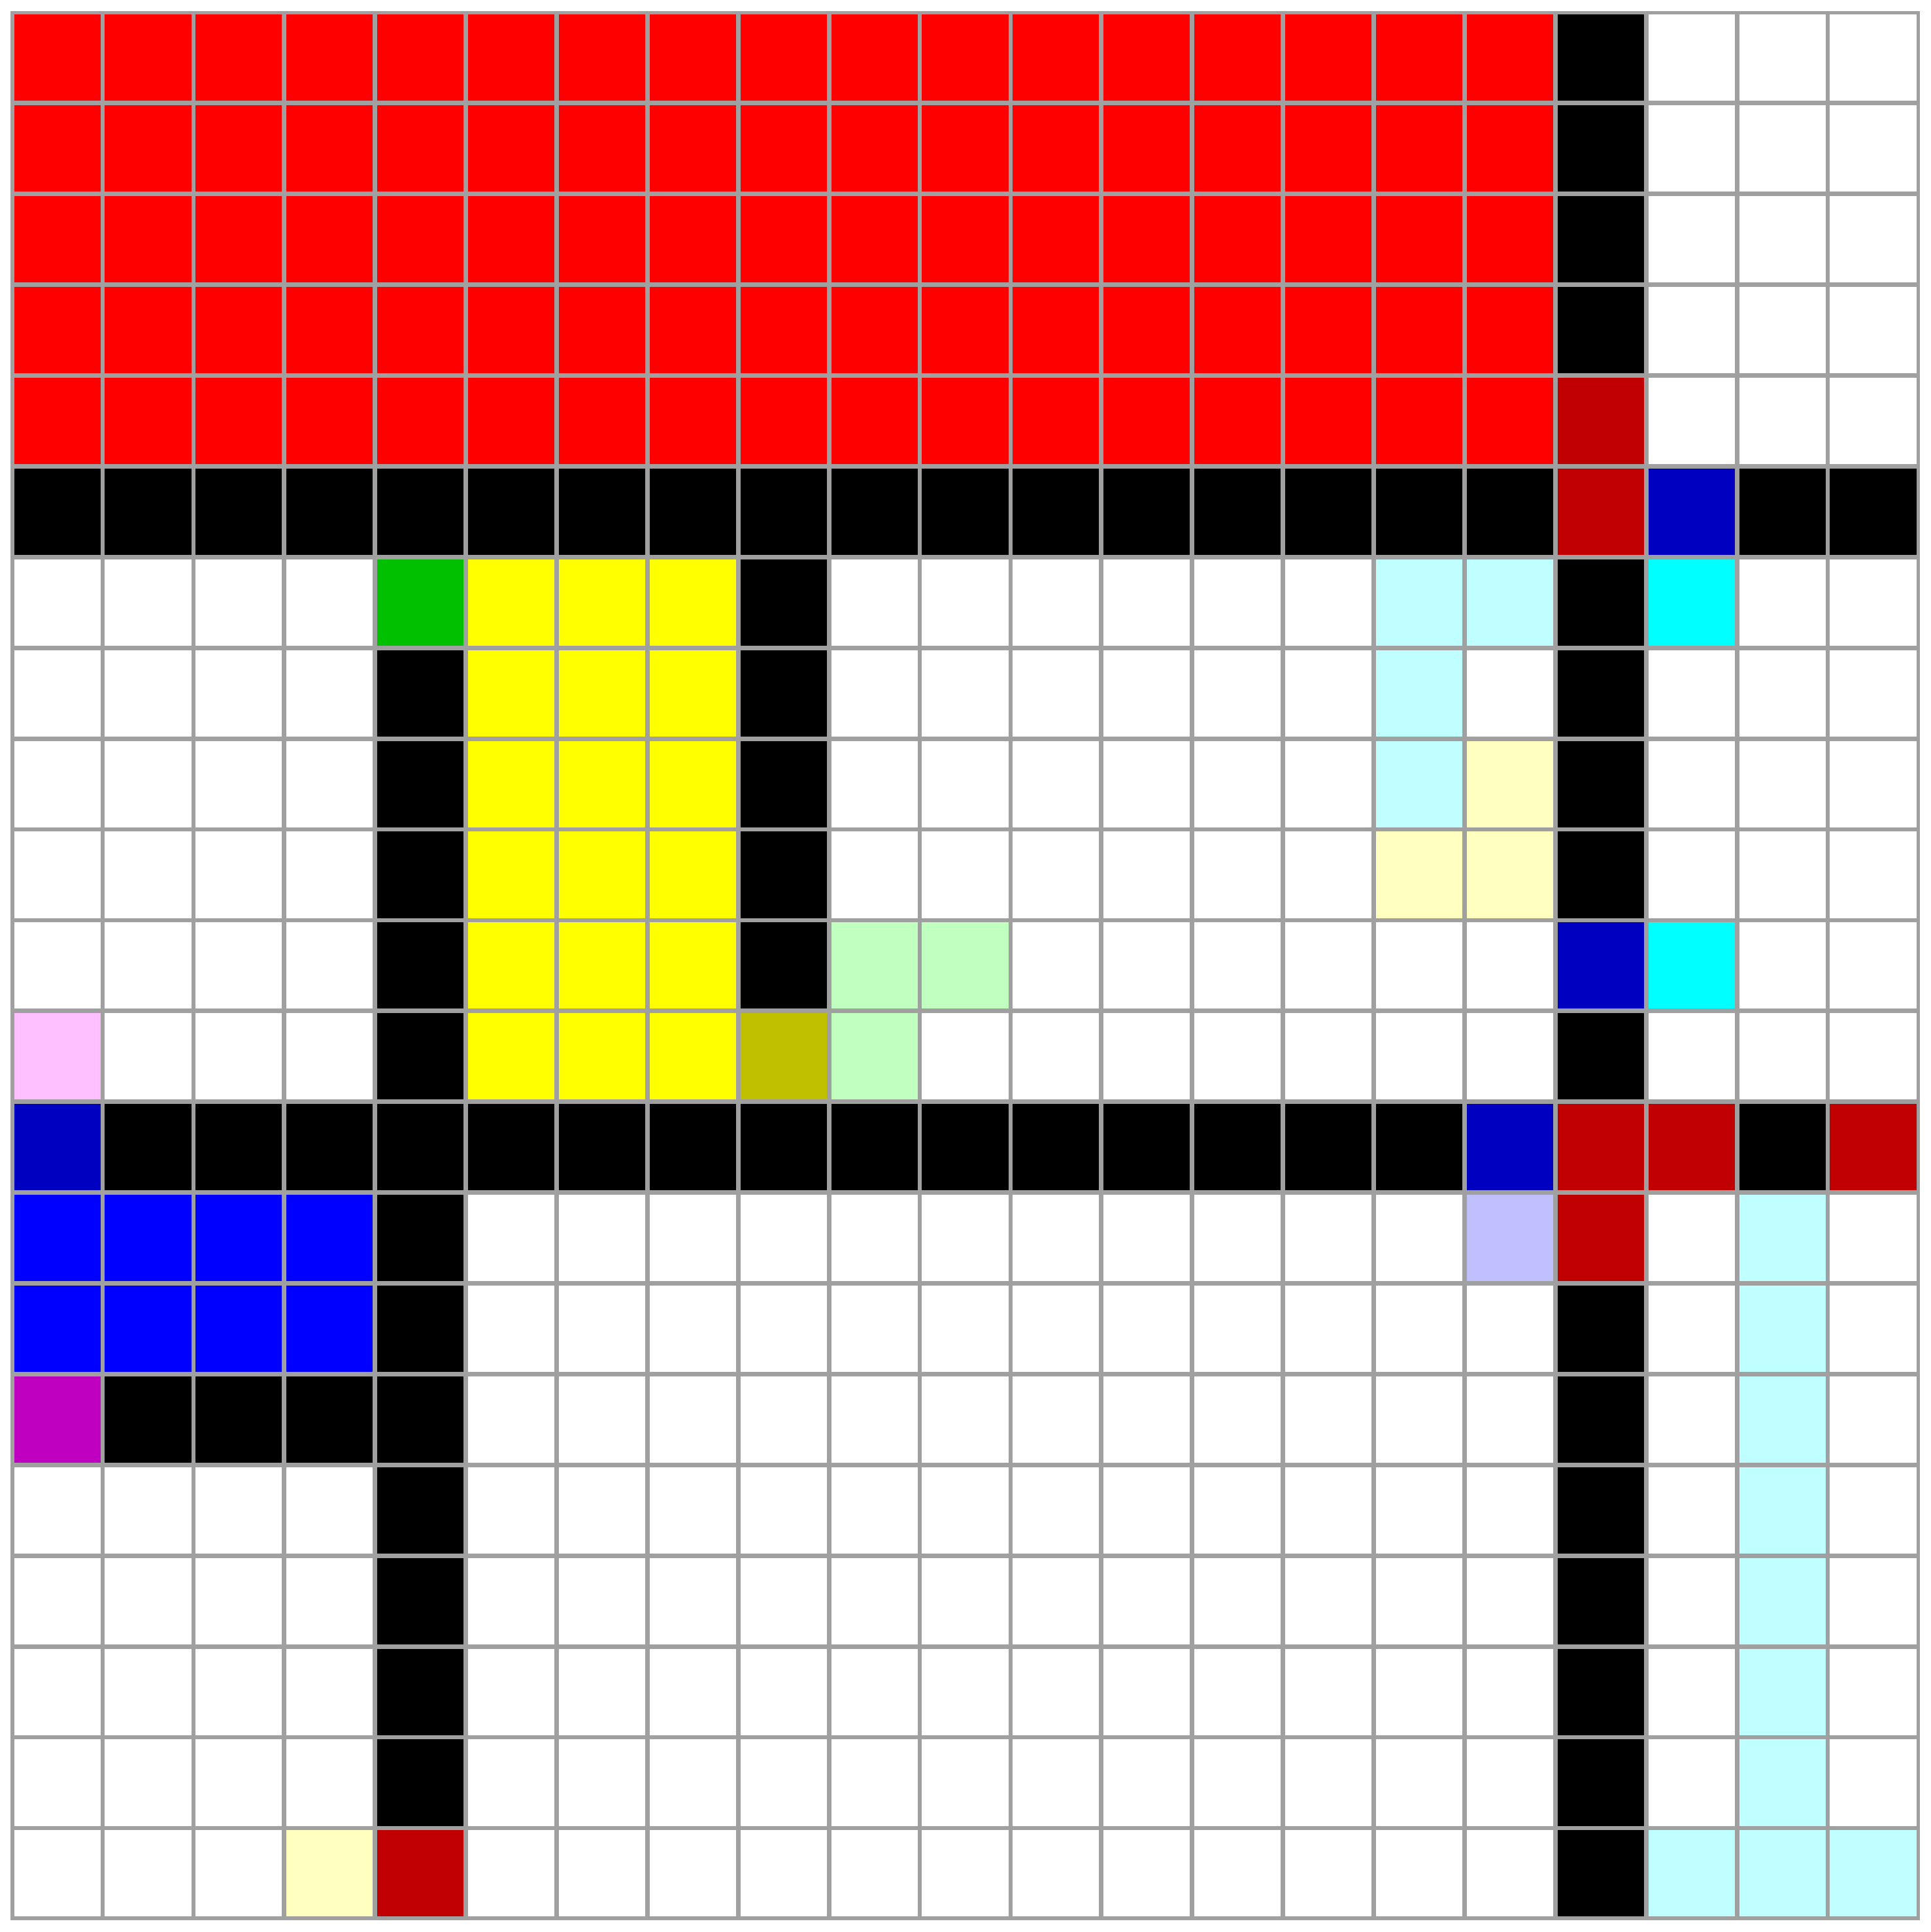
\includegraphics[width=0.6\linewidth]{utmc_composition.eps}
\end{center}

芸術的ですね。カラーだと左上が赤、真ん中が黄色、左下が青なのでまさしく「赤・青・黄のコンポジション」なんですが……。モノクロではわかんないですね。

どこがどうなって "UTMC" と出力されるのかわからない人向けに、インタプリタの軌跡を矢印で表してみました\footnote{Excel実装の面目躍如!}。

\begin{center}
	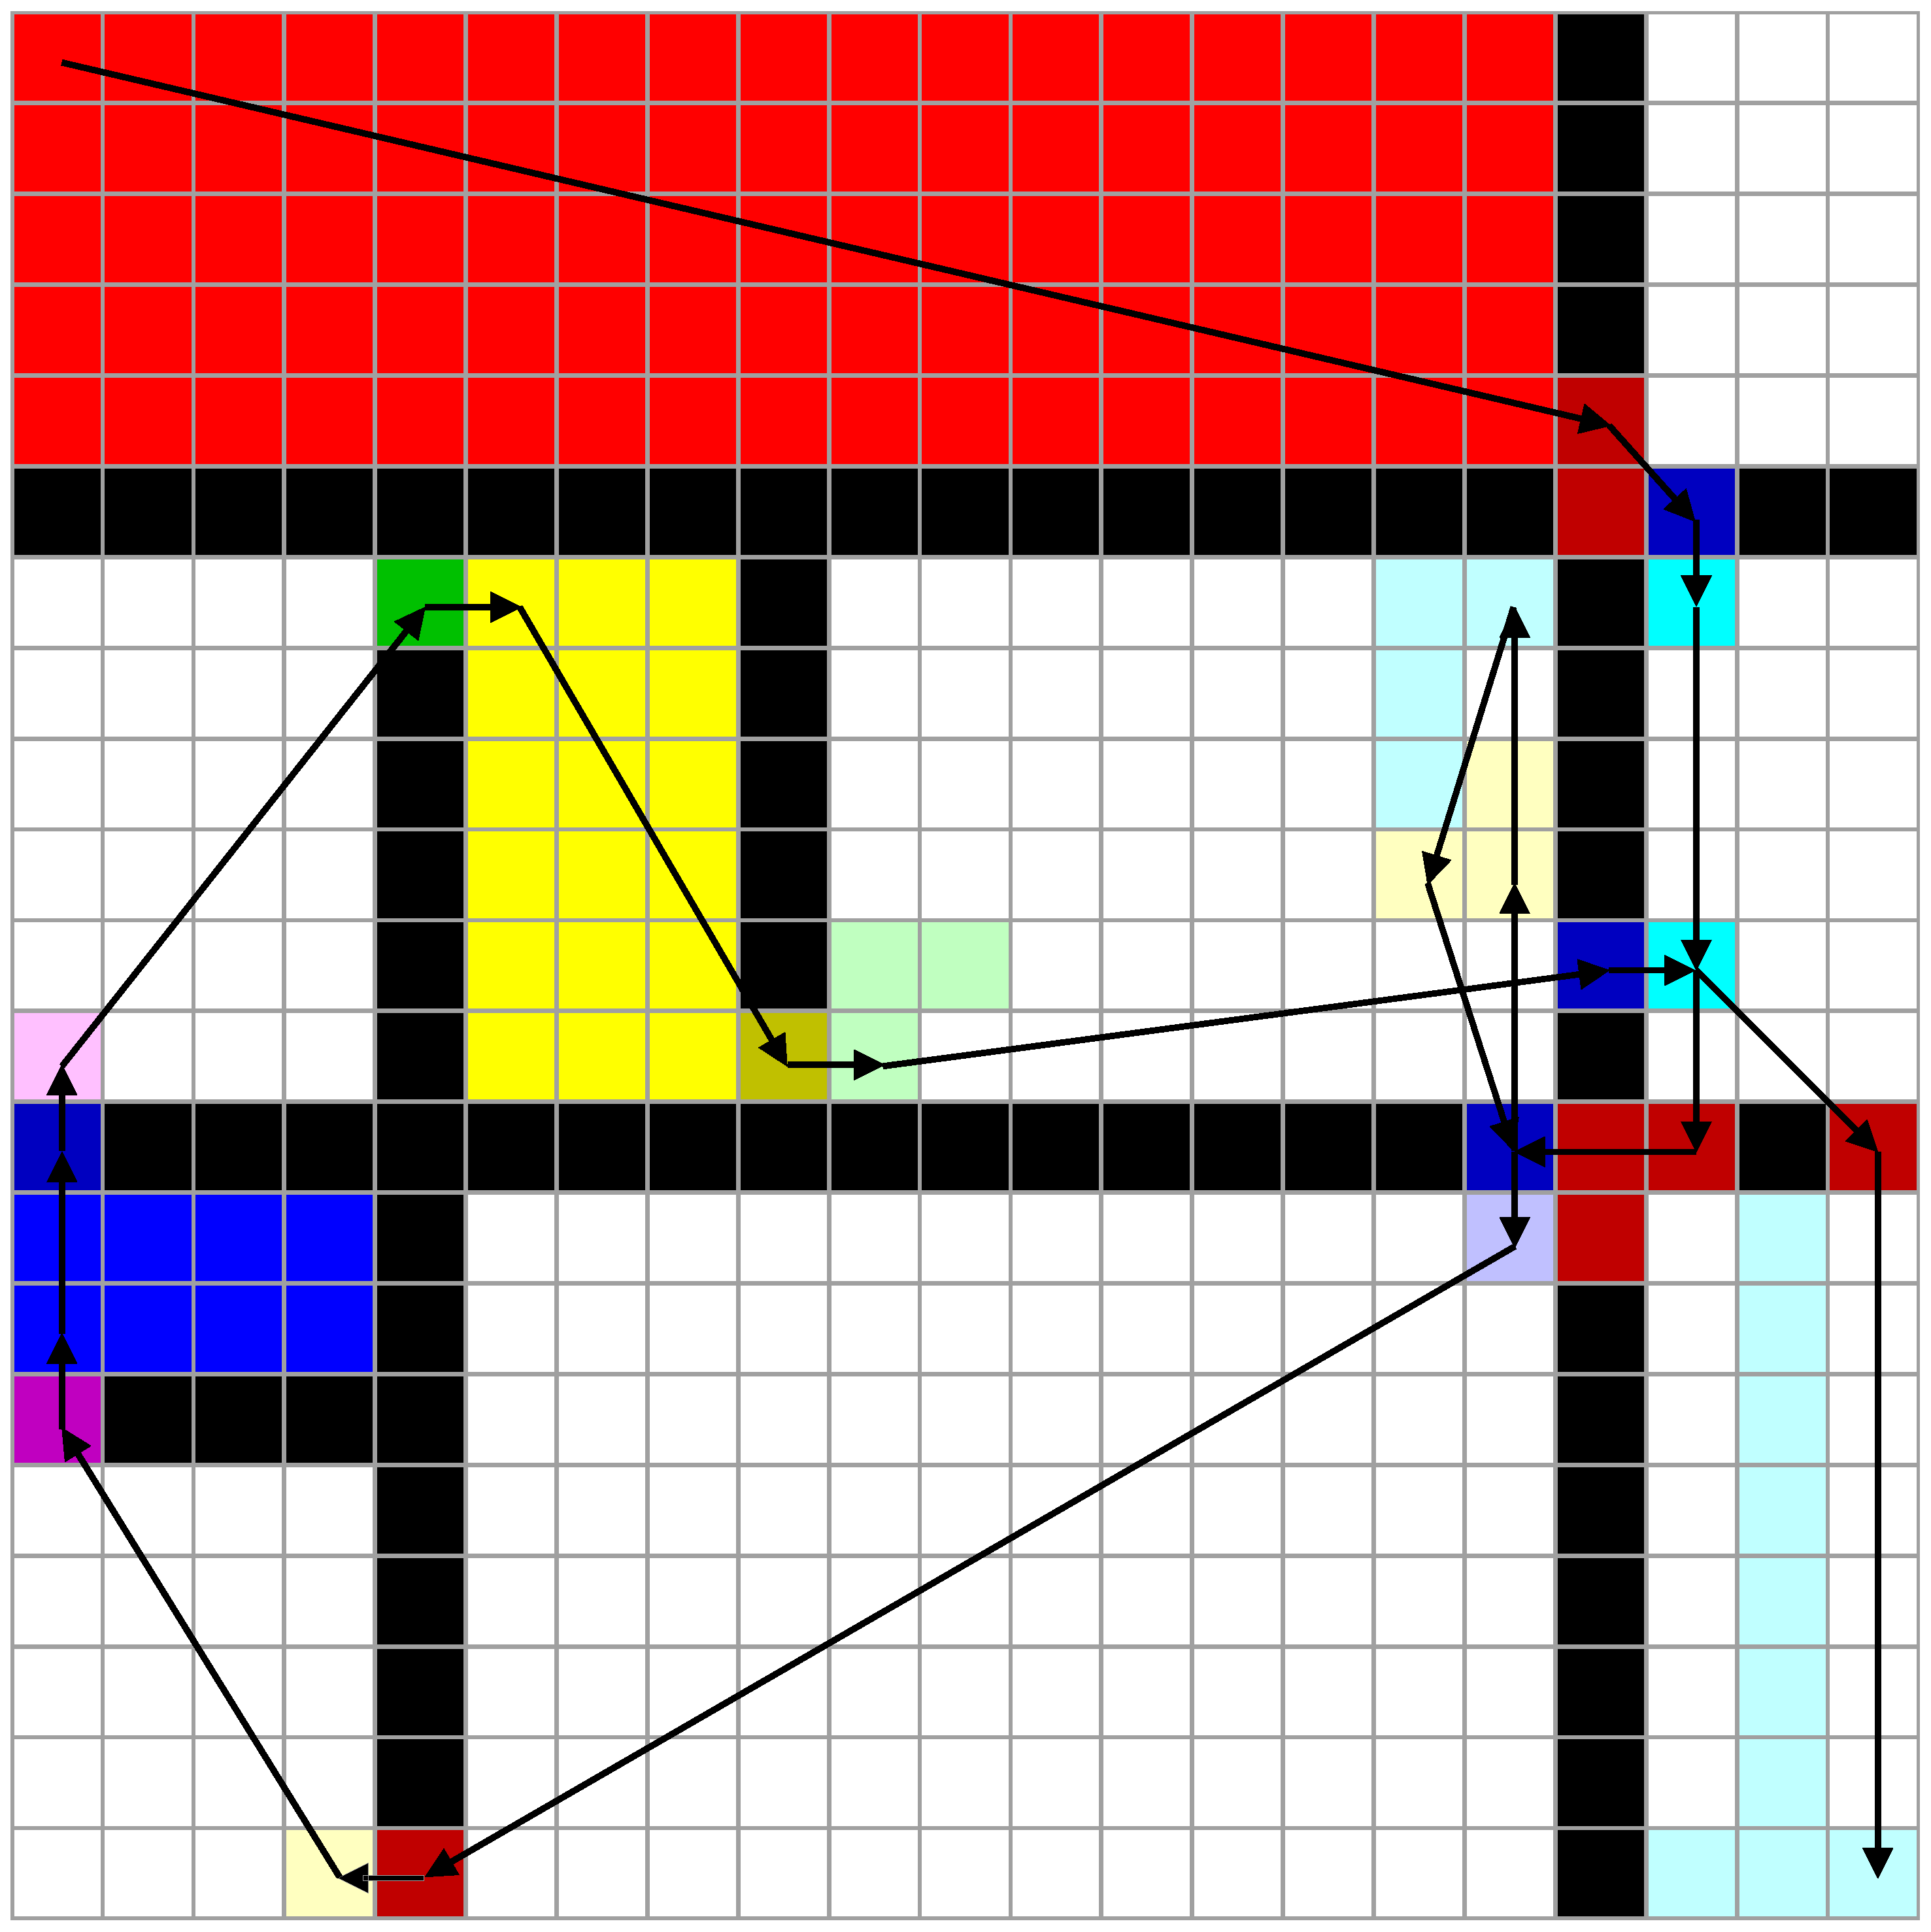
\includegraphics[width=0.6\linewidth]{utmc_composition_trace.eps}
\end{center}

上段で85をスタックに積み、"U" (Unicode値85) を出力。中段までで85を3回複製して下段で85から1を引き、 "T" (84) を出力。下段左端で85から8を引いて "M" (77) を出力、中段に戻って85から18を引き "C" (67) を出力、右下に入ってプログラム終了、という流れです。

\subsection{UTMCロゴ}
現代芸術はわからないという方向けに、別の見た目のコードも用意してみました。弊サークルのロゴマークです。

\begin{center}
	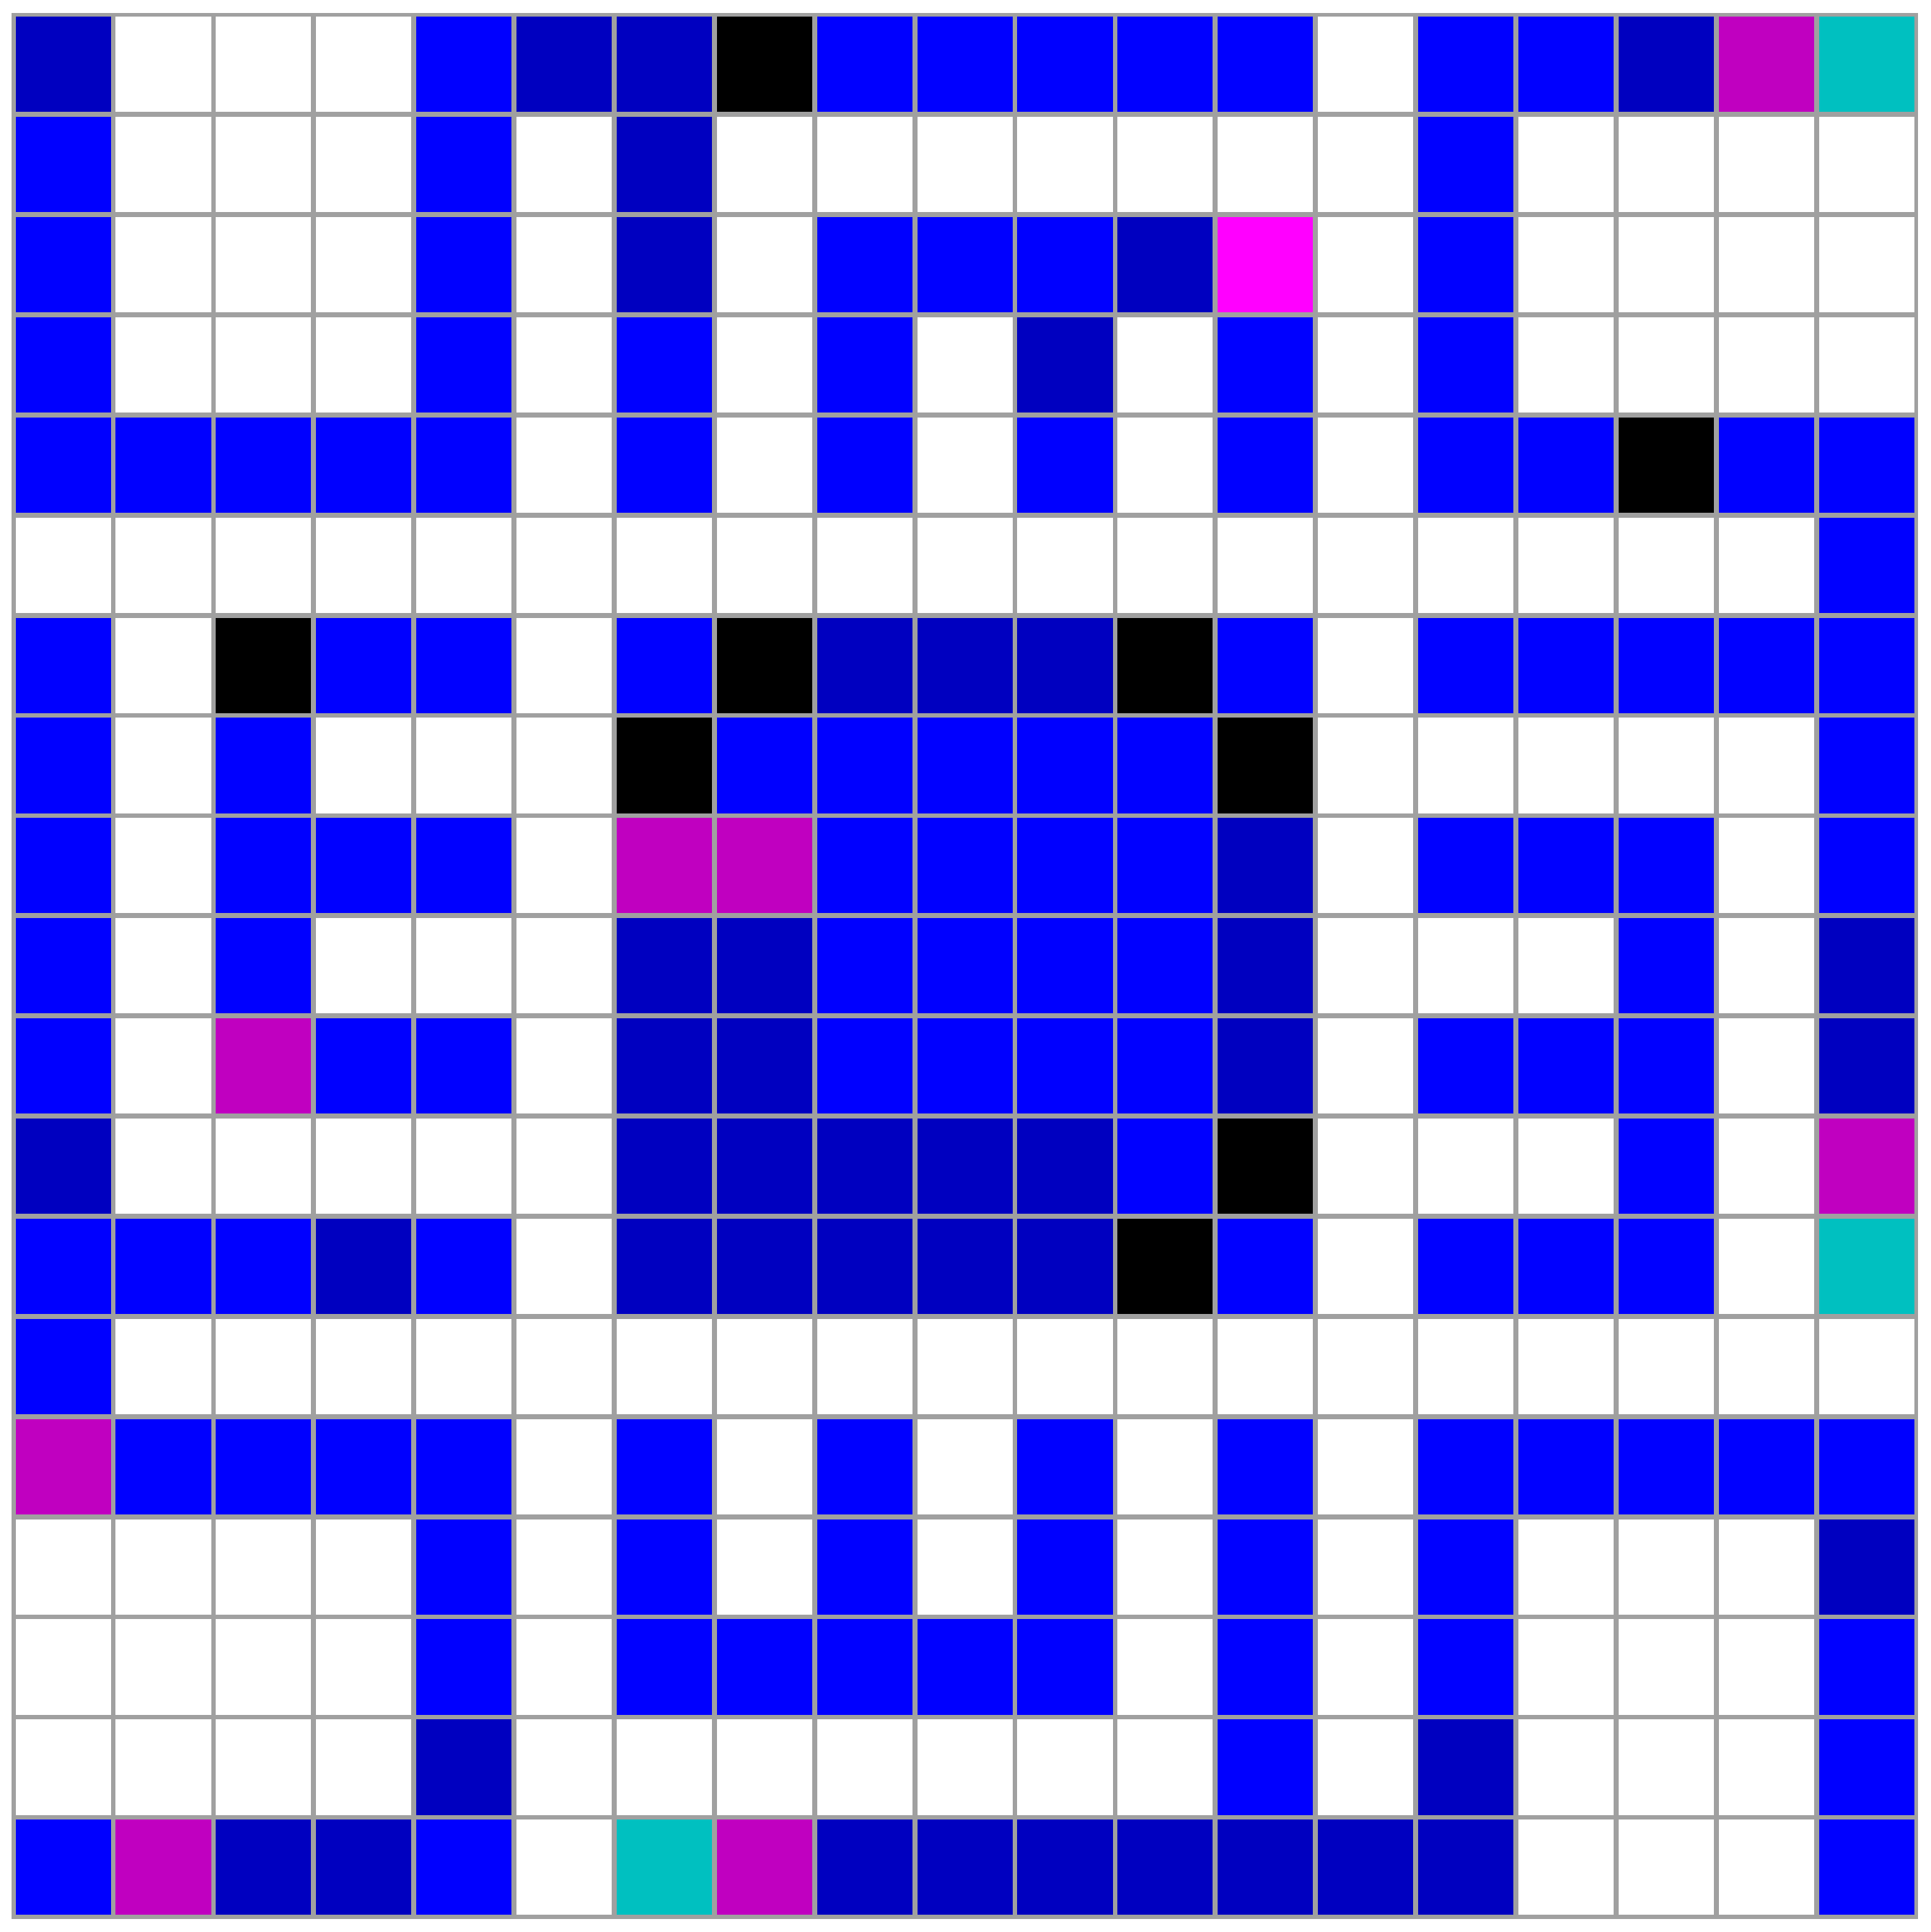
\includegraphics[width=0.6\linewidth]{utmc_logo.eps}
\end{center}

これも "UTMC" と出力するコードです。\footnote{There's More Than One Way To Do It!}

こちらもトレース結果を置いておきます。

\begin{center}
	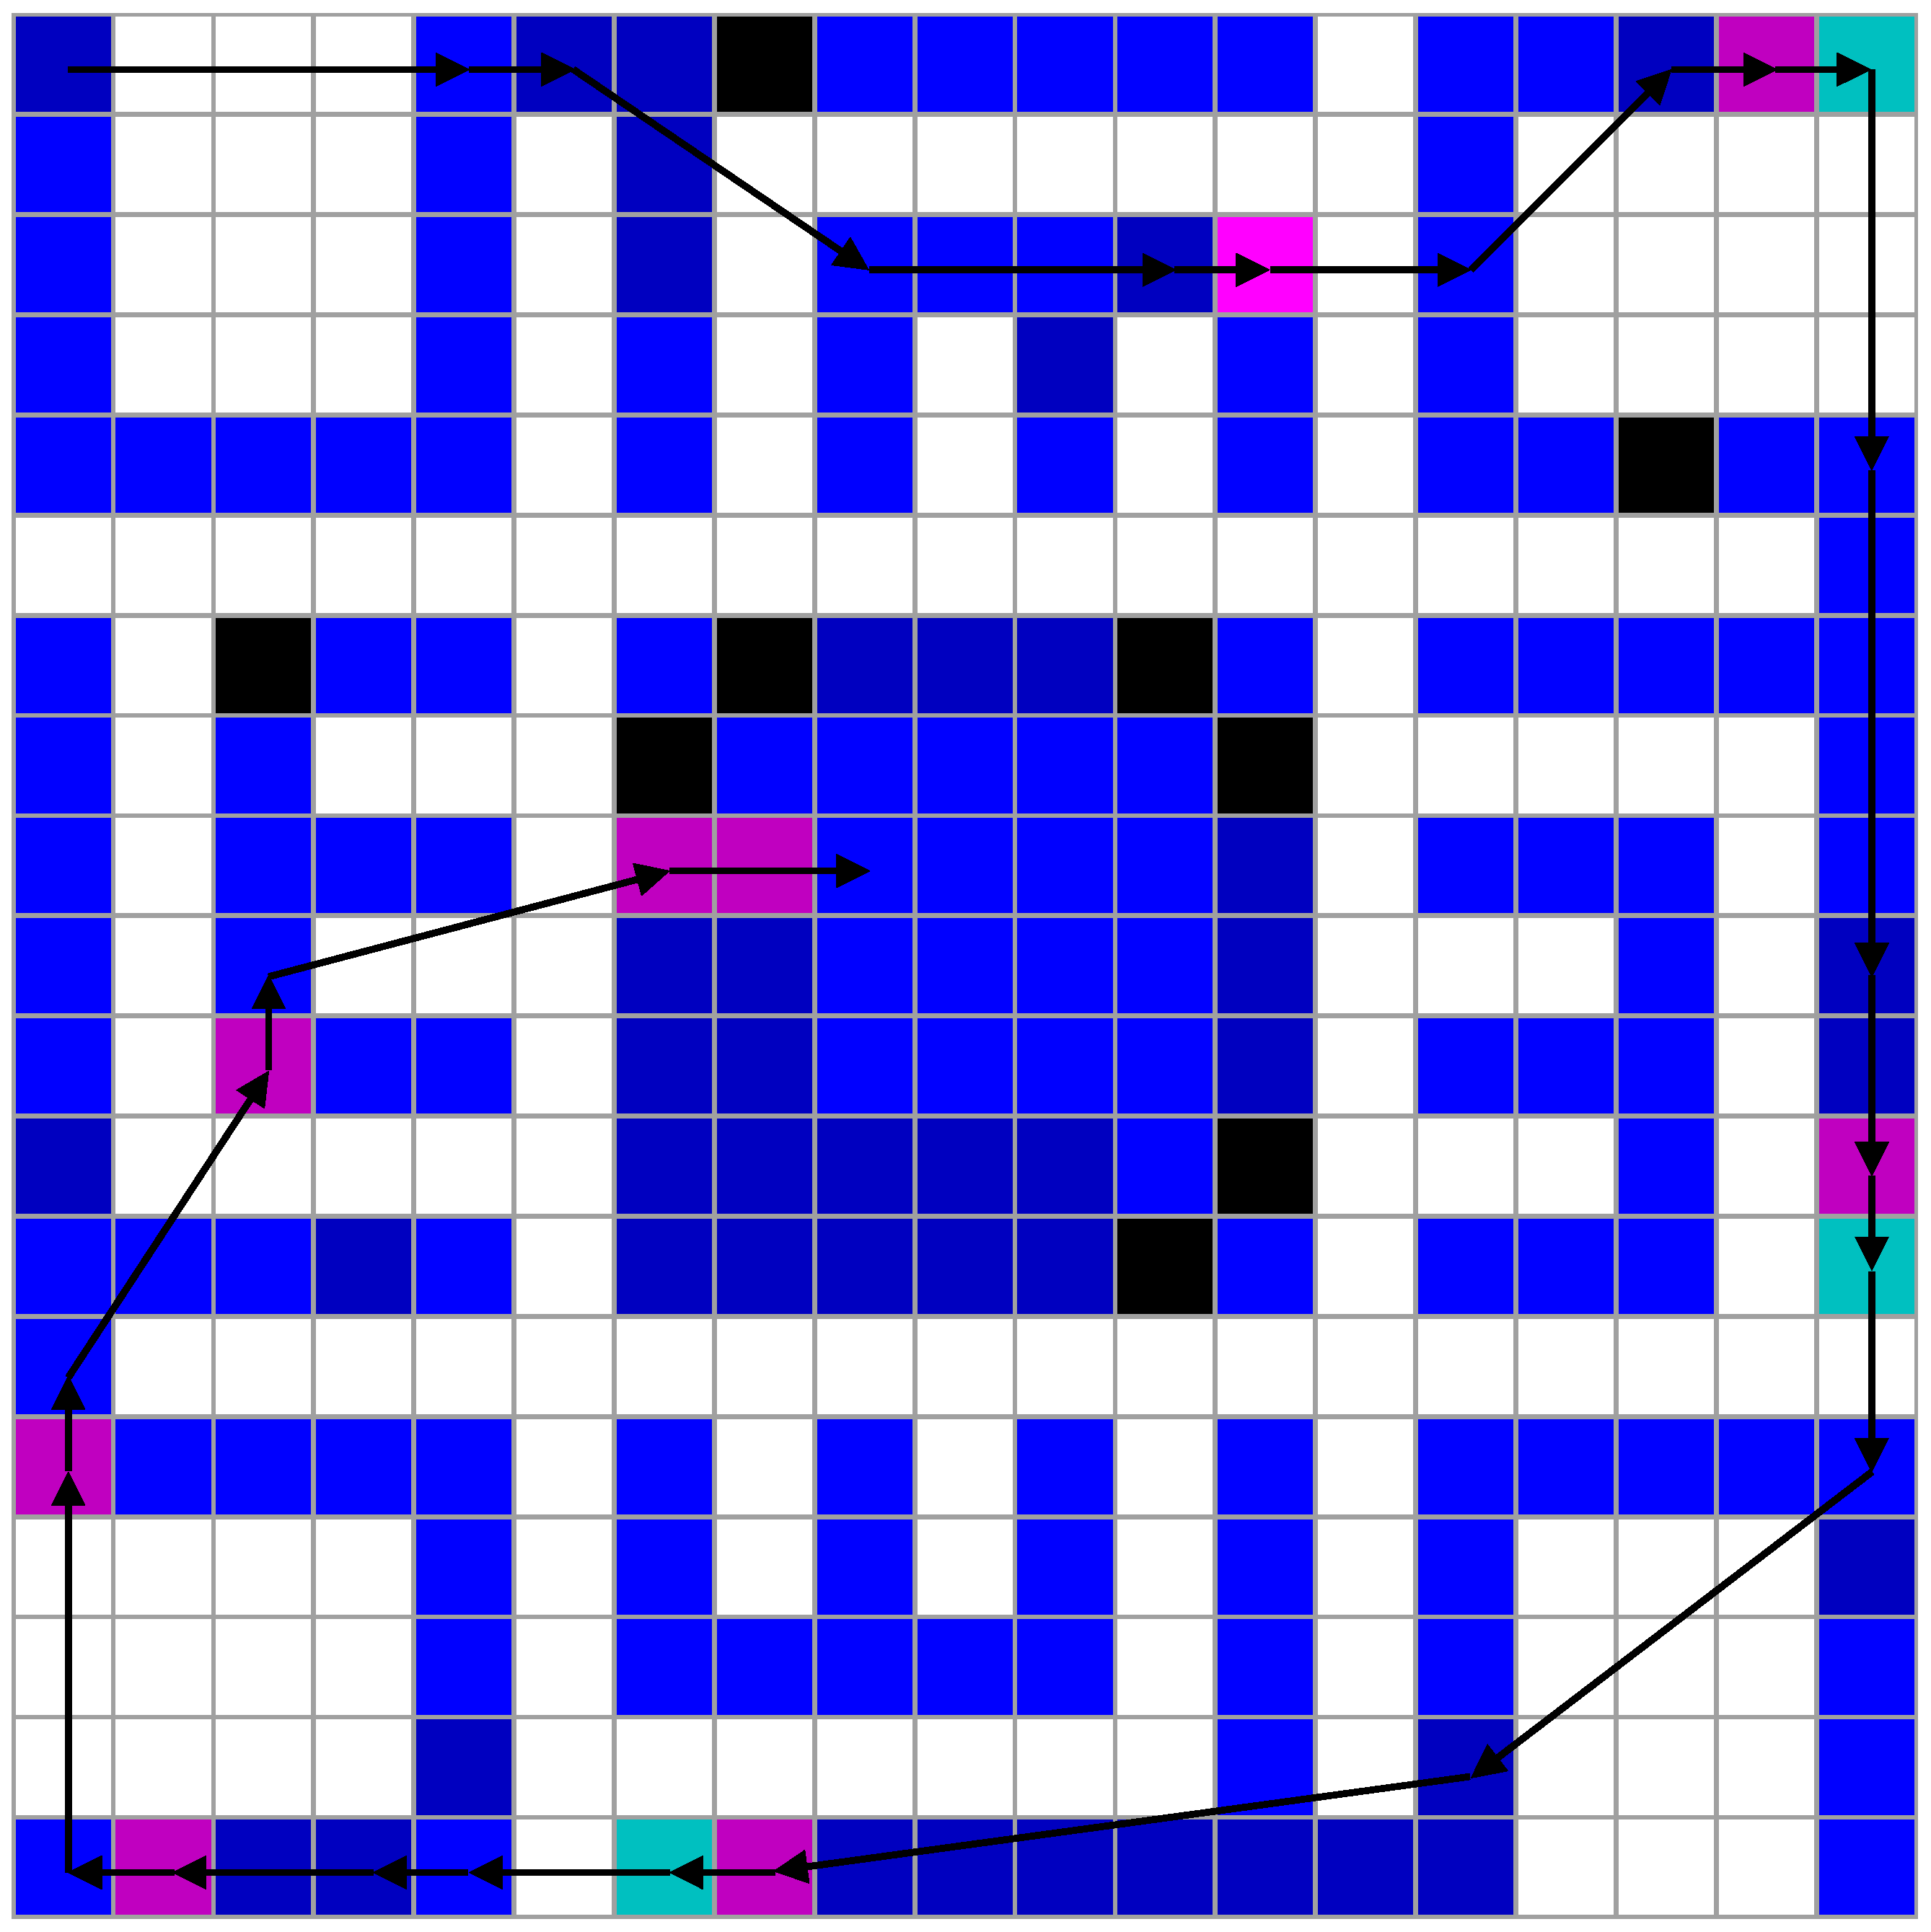
\includegraphics[width=0.6\linewidth]{utmc_logo_trace.eps}
\end{center}

時計回りにぐるっと1周しているだけなので軌跡はさっきよりもわかりやすいですね。

今度は "C", "M", "T", "U" の順にスタックに積んでから一気に出力しています。全体を青でほぼ統一し、他の有彩色はシアン・マゼンタにとどめてみたのですが、コーディングできる領域がほぼ全て幅1の線なのもあってなかなか難しかったです。

\subsection{FizzBuzz}
もうちょっと歯ごたえのあるプログラムとして、FizzBuzz\footnote{1, 2, Fizz, 4, Buzz, Fizz, 7, ...というように、1から順番にカウントアップしていって、3の倍数のときはFizz、5の倍数のときはBuzz、15の倍数のときはFizzBuzz、それ以外のときは数字を言う遊びです。}も書いてみました。100以下の数字に対して出力します。

\begin{center}
	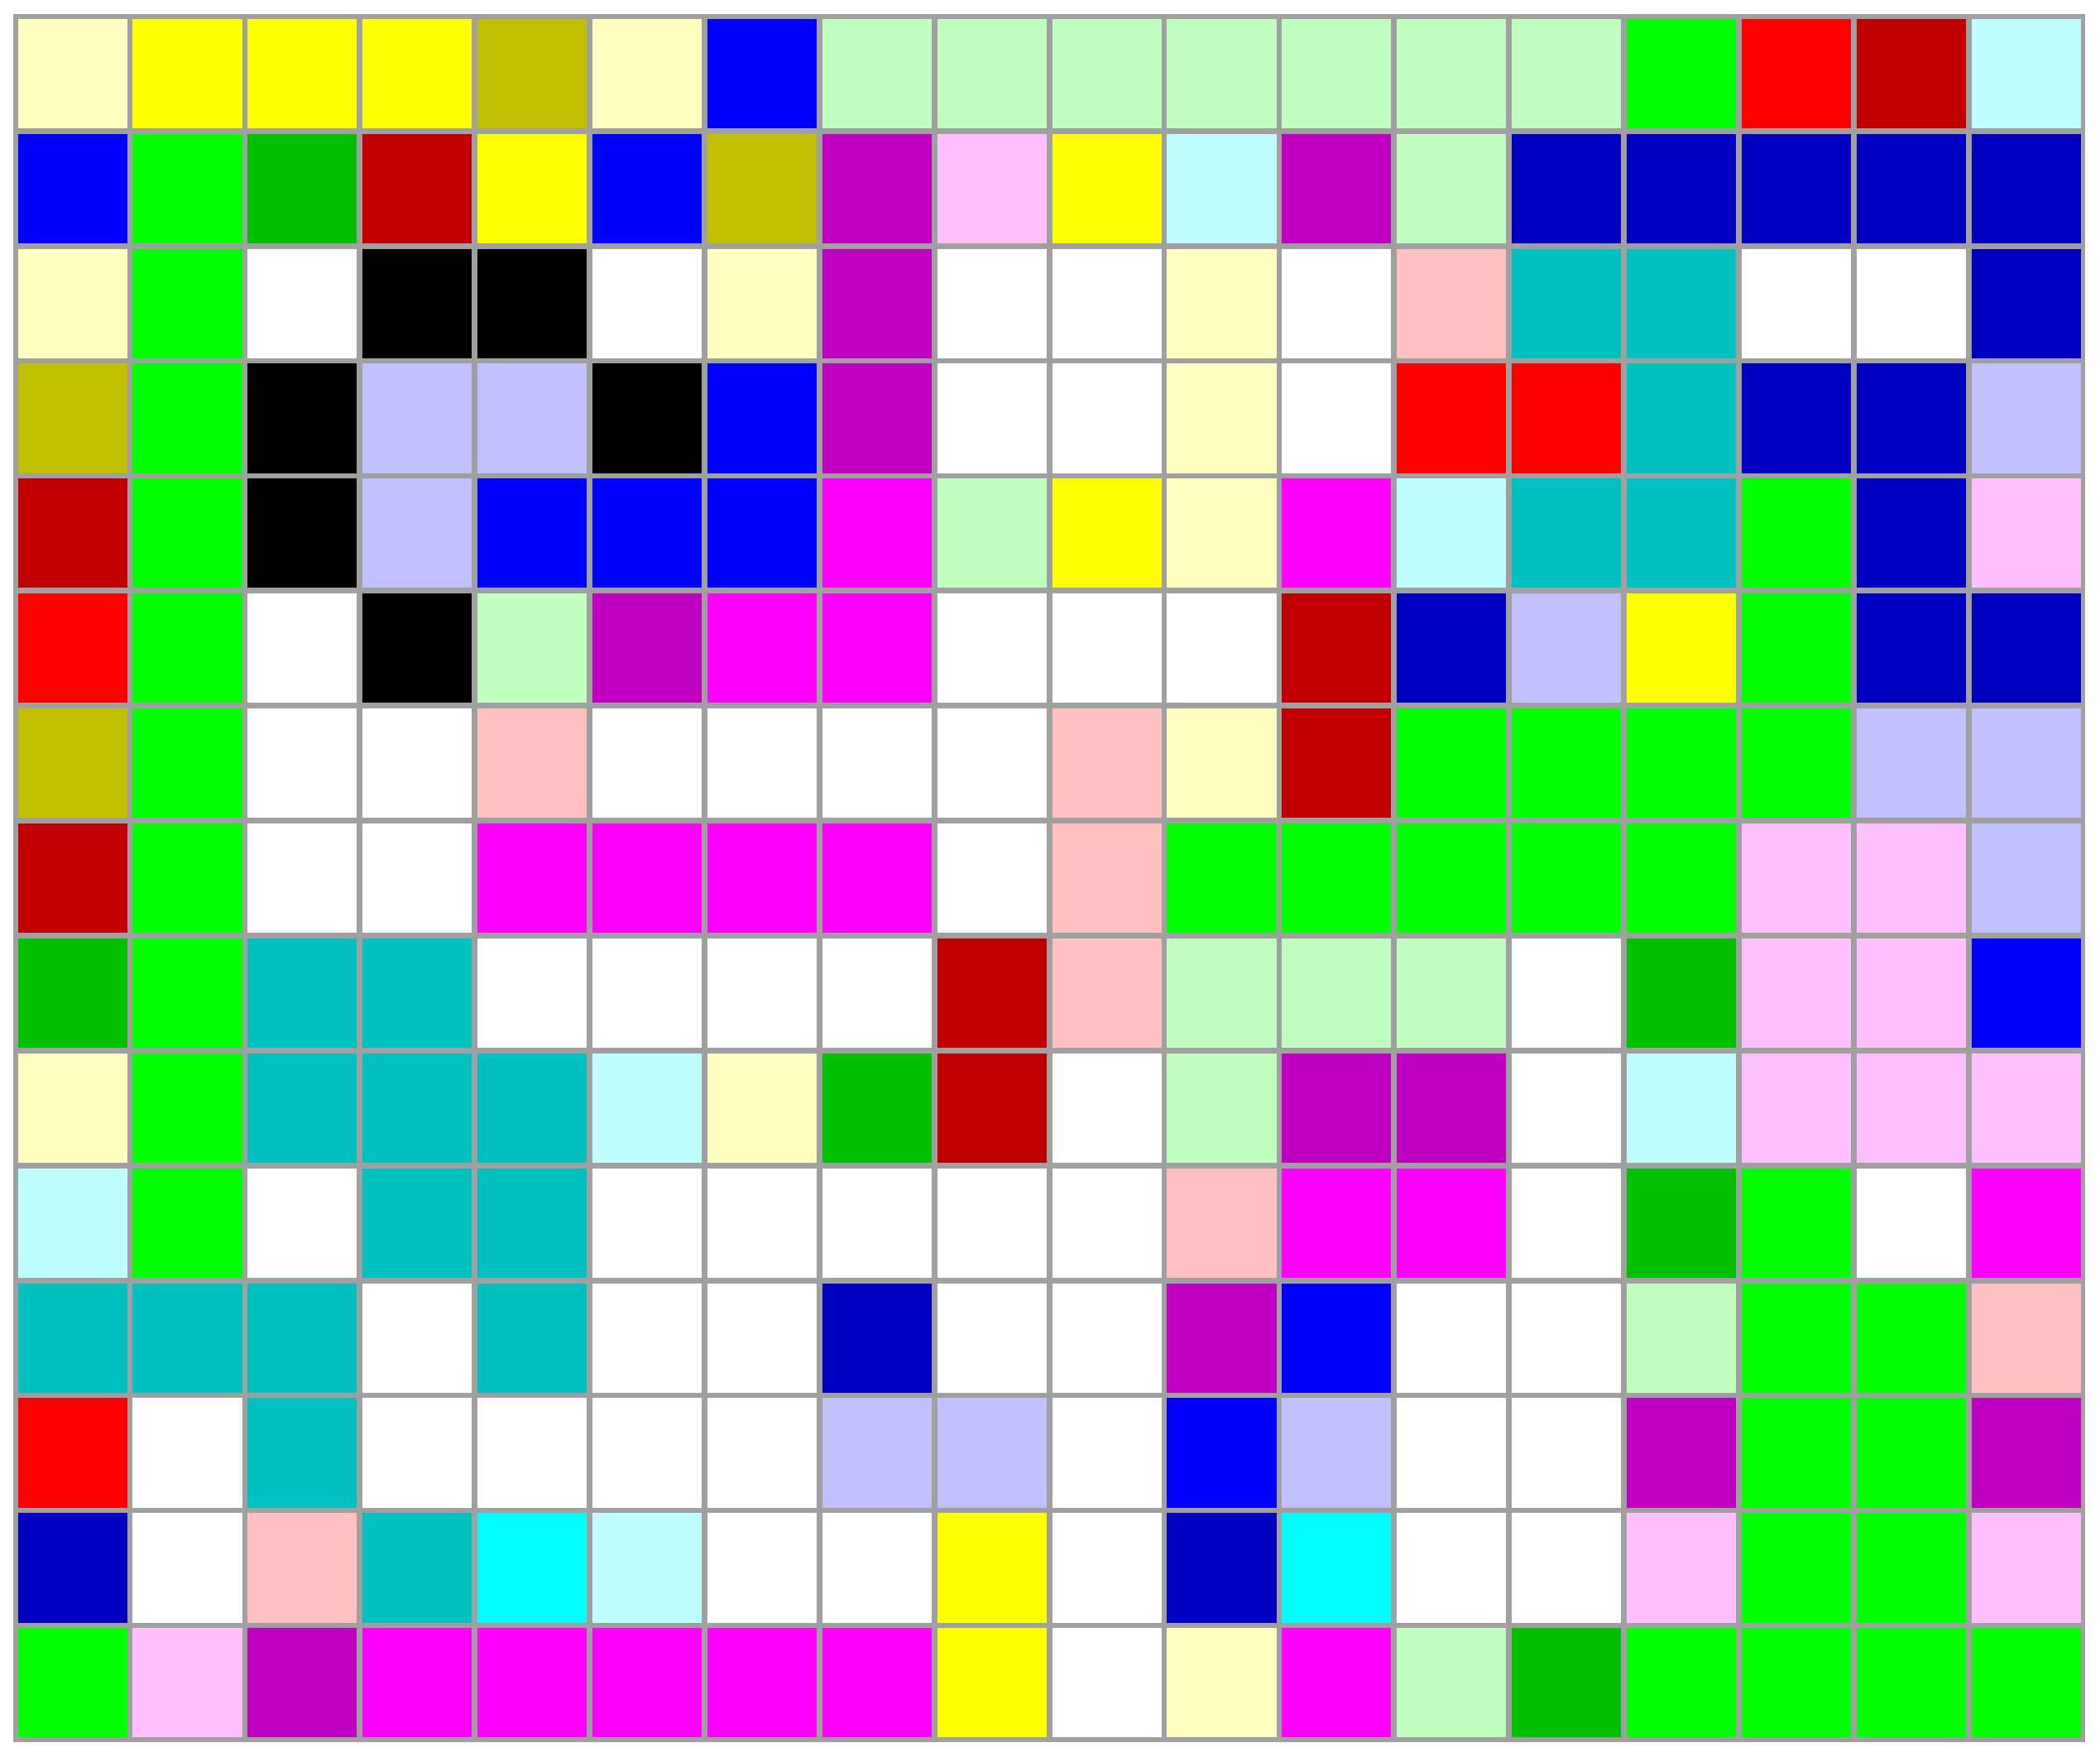
\includegraphics[width=0.6\linewidth]{fizzbuzz.eps}
\end{center}

このレベルで見た目にこだわってるとソースコードの大きさがとてつもないことになるので、なるべく小さく作ることに主眼を置きました。もはやただのモザイクです。

\begin{center}
	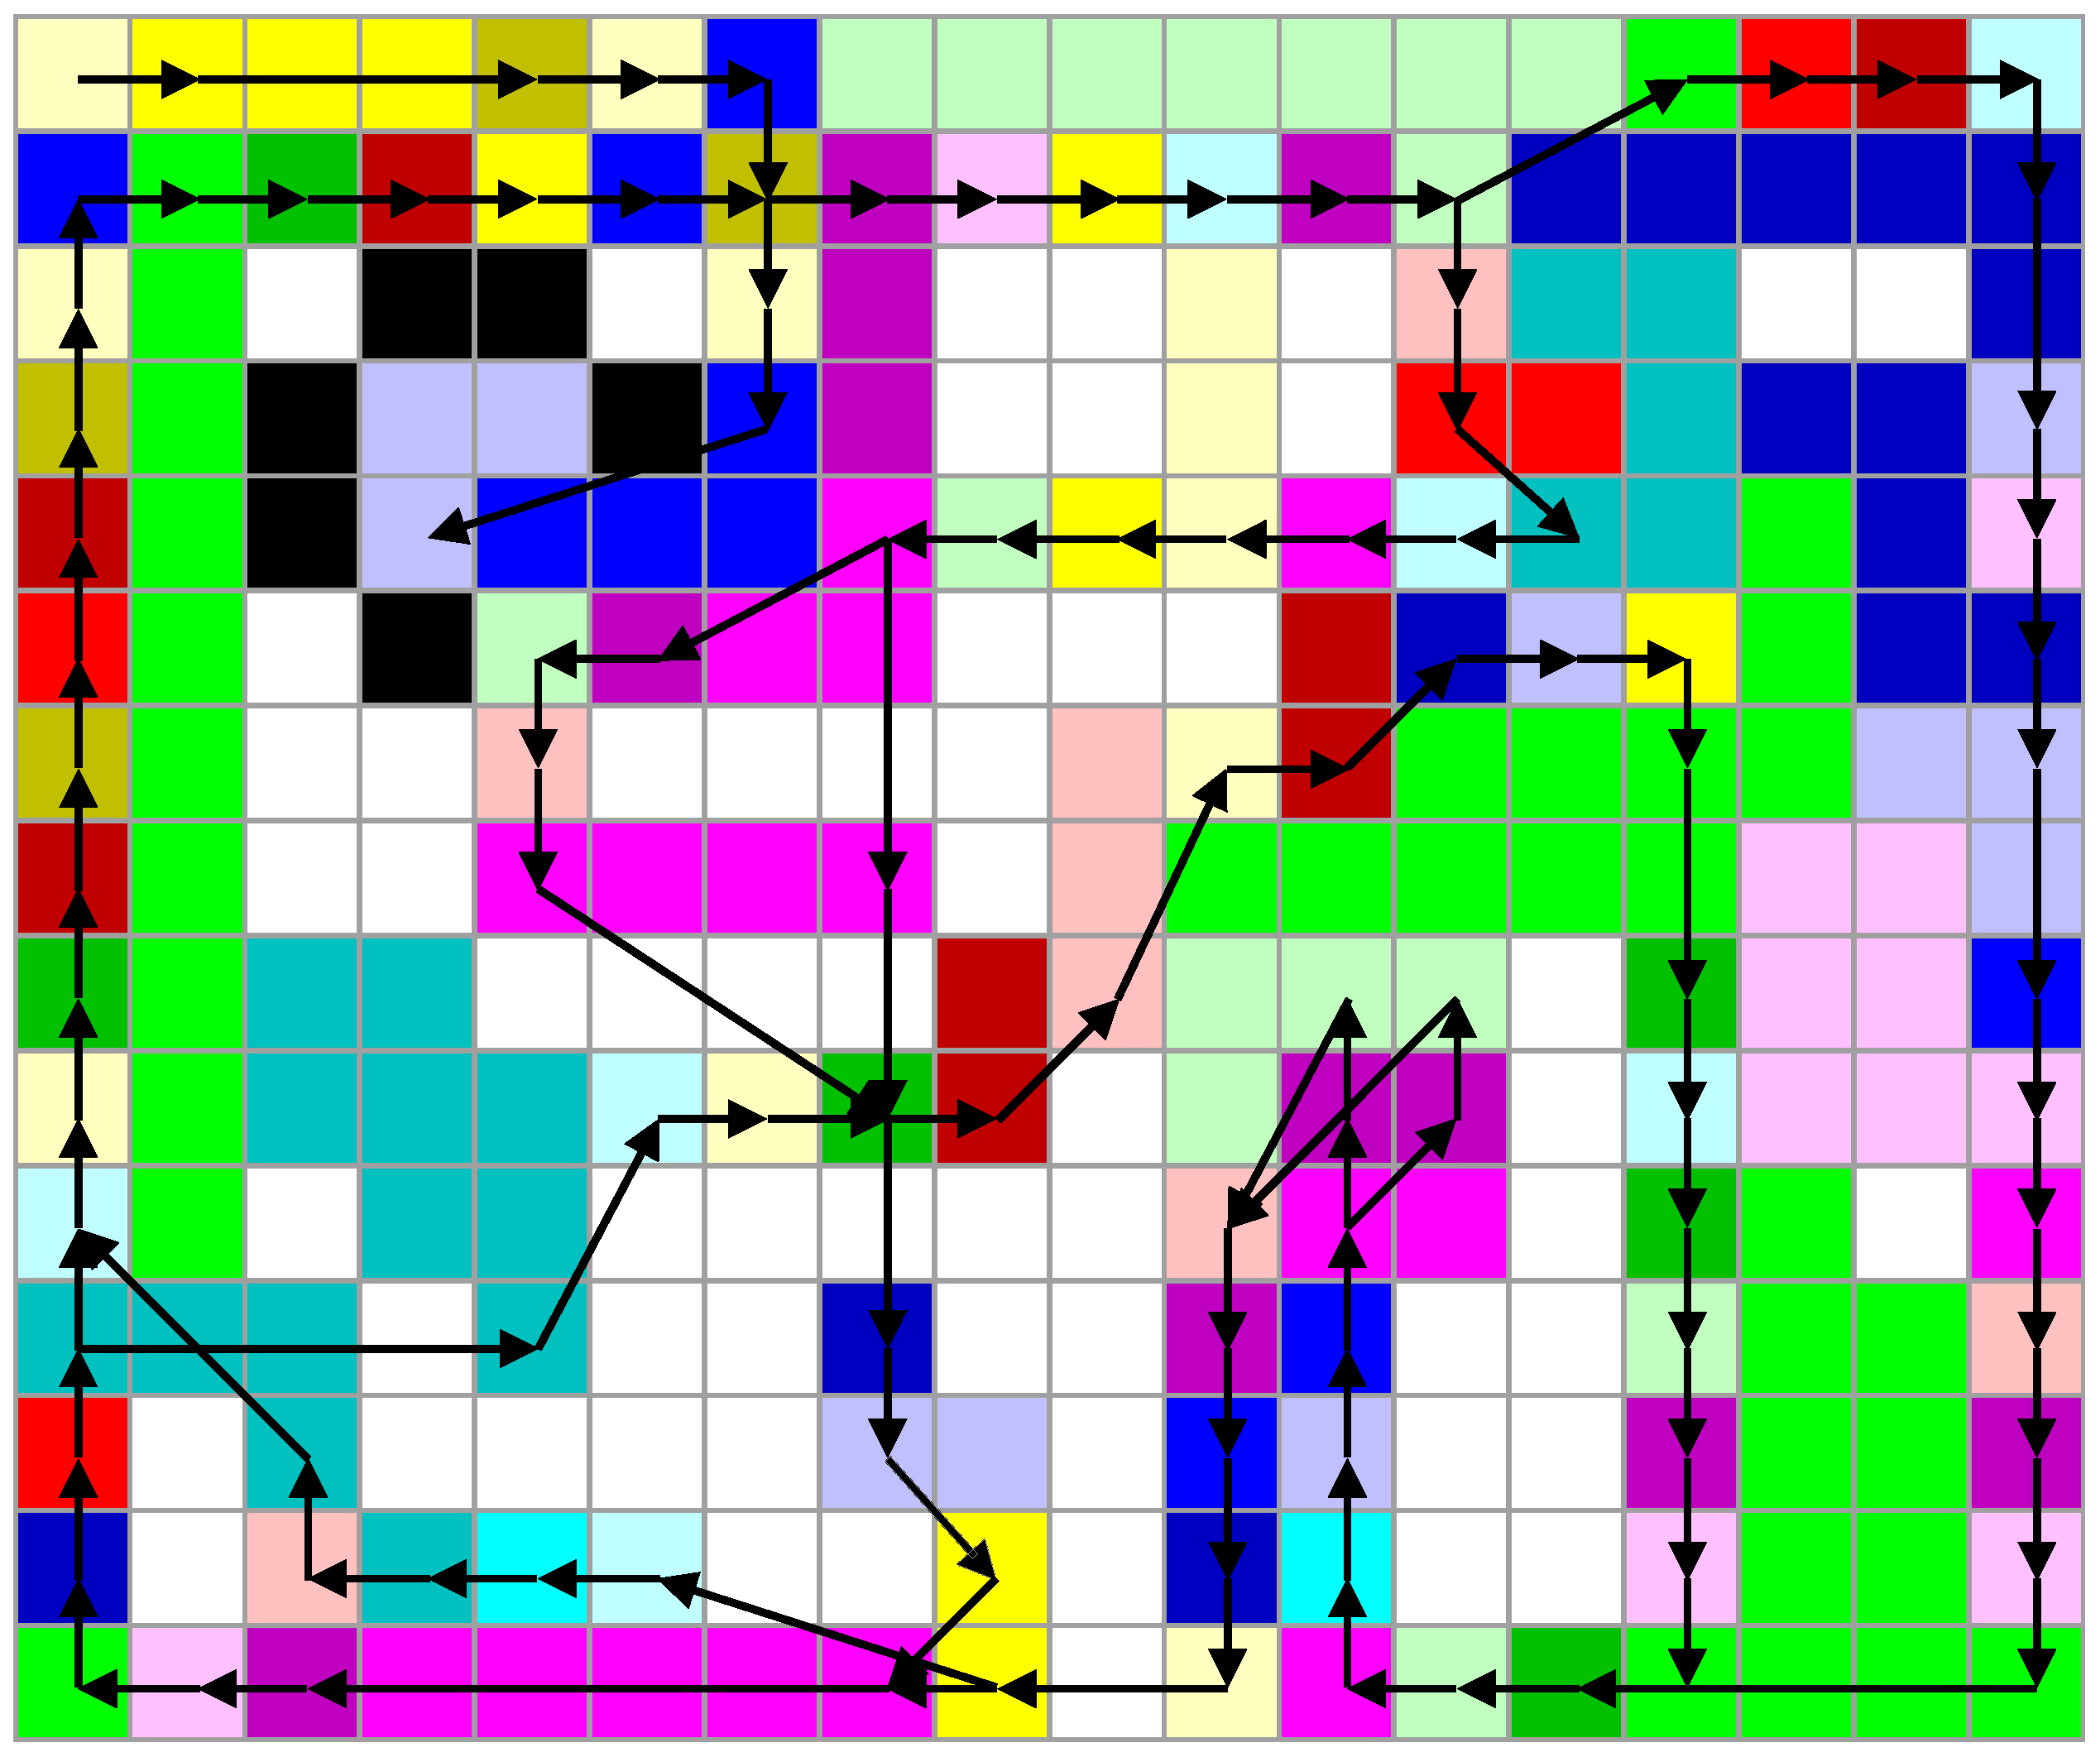
\includegraphics[width=0.6\linewidth]{fizzbuzz_trace.eps}
\end{center}

トレース見てもわけがわかりませんね。もうちょっと詳しく説明してみます。

\begin{center}
	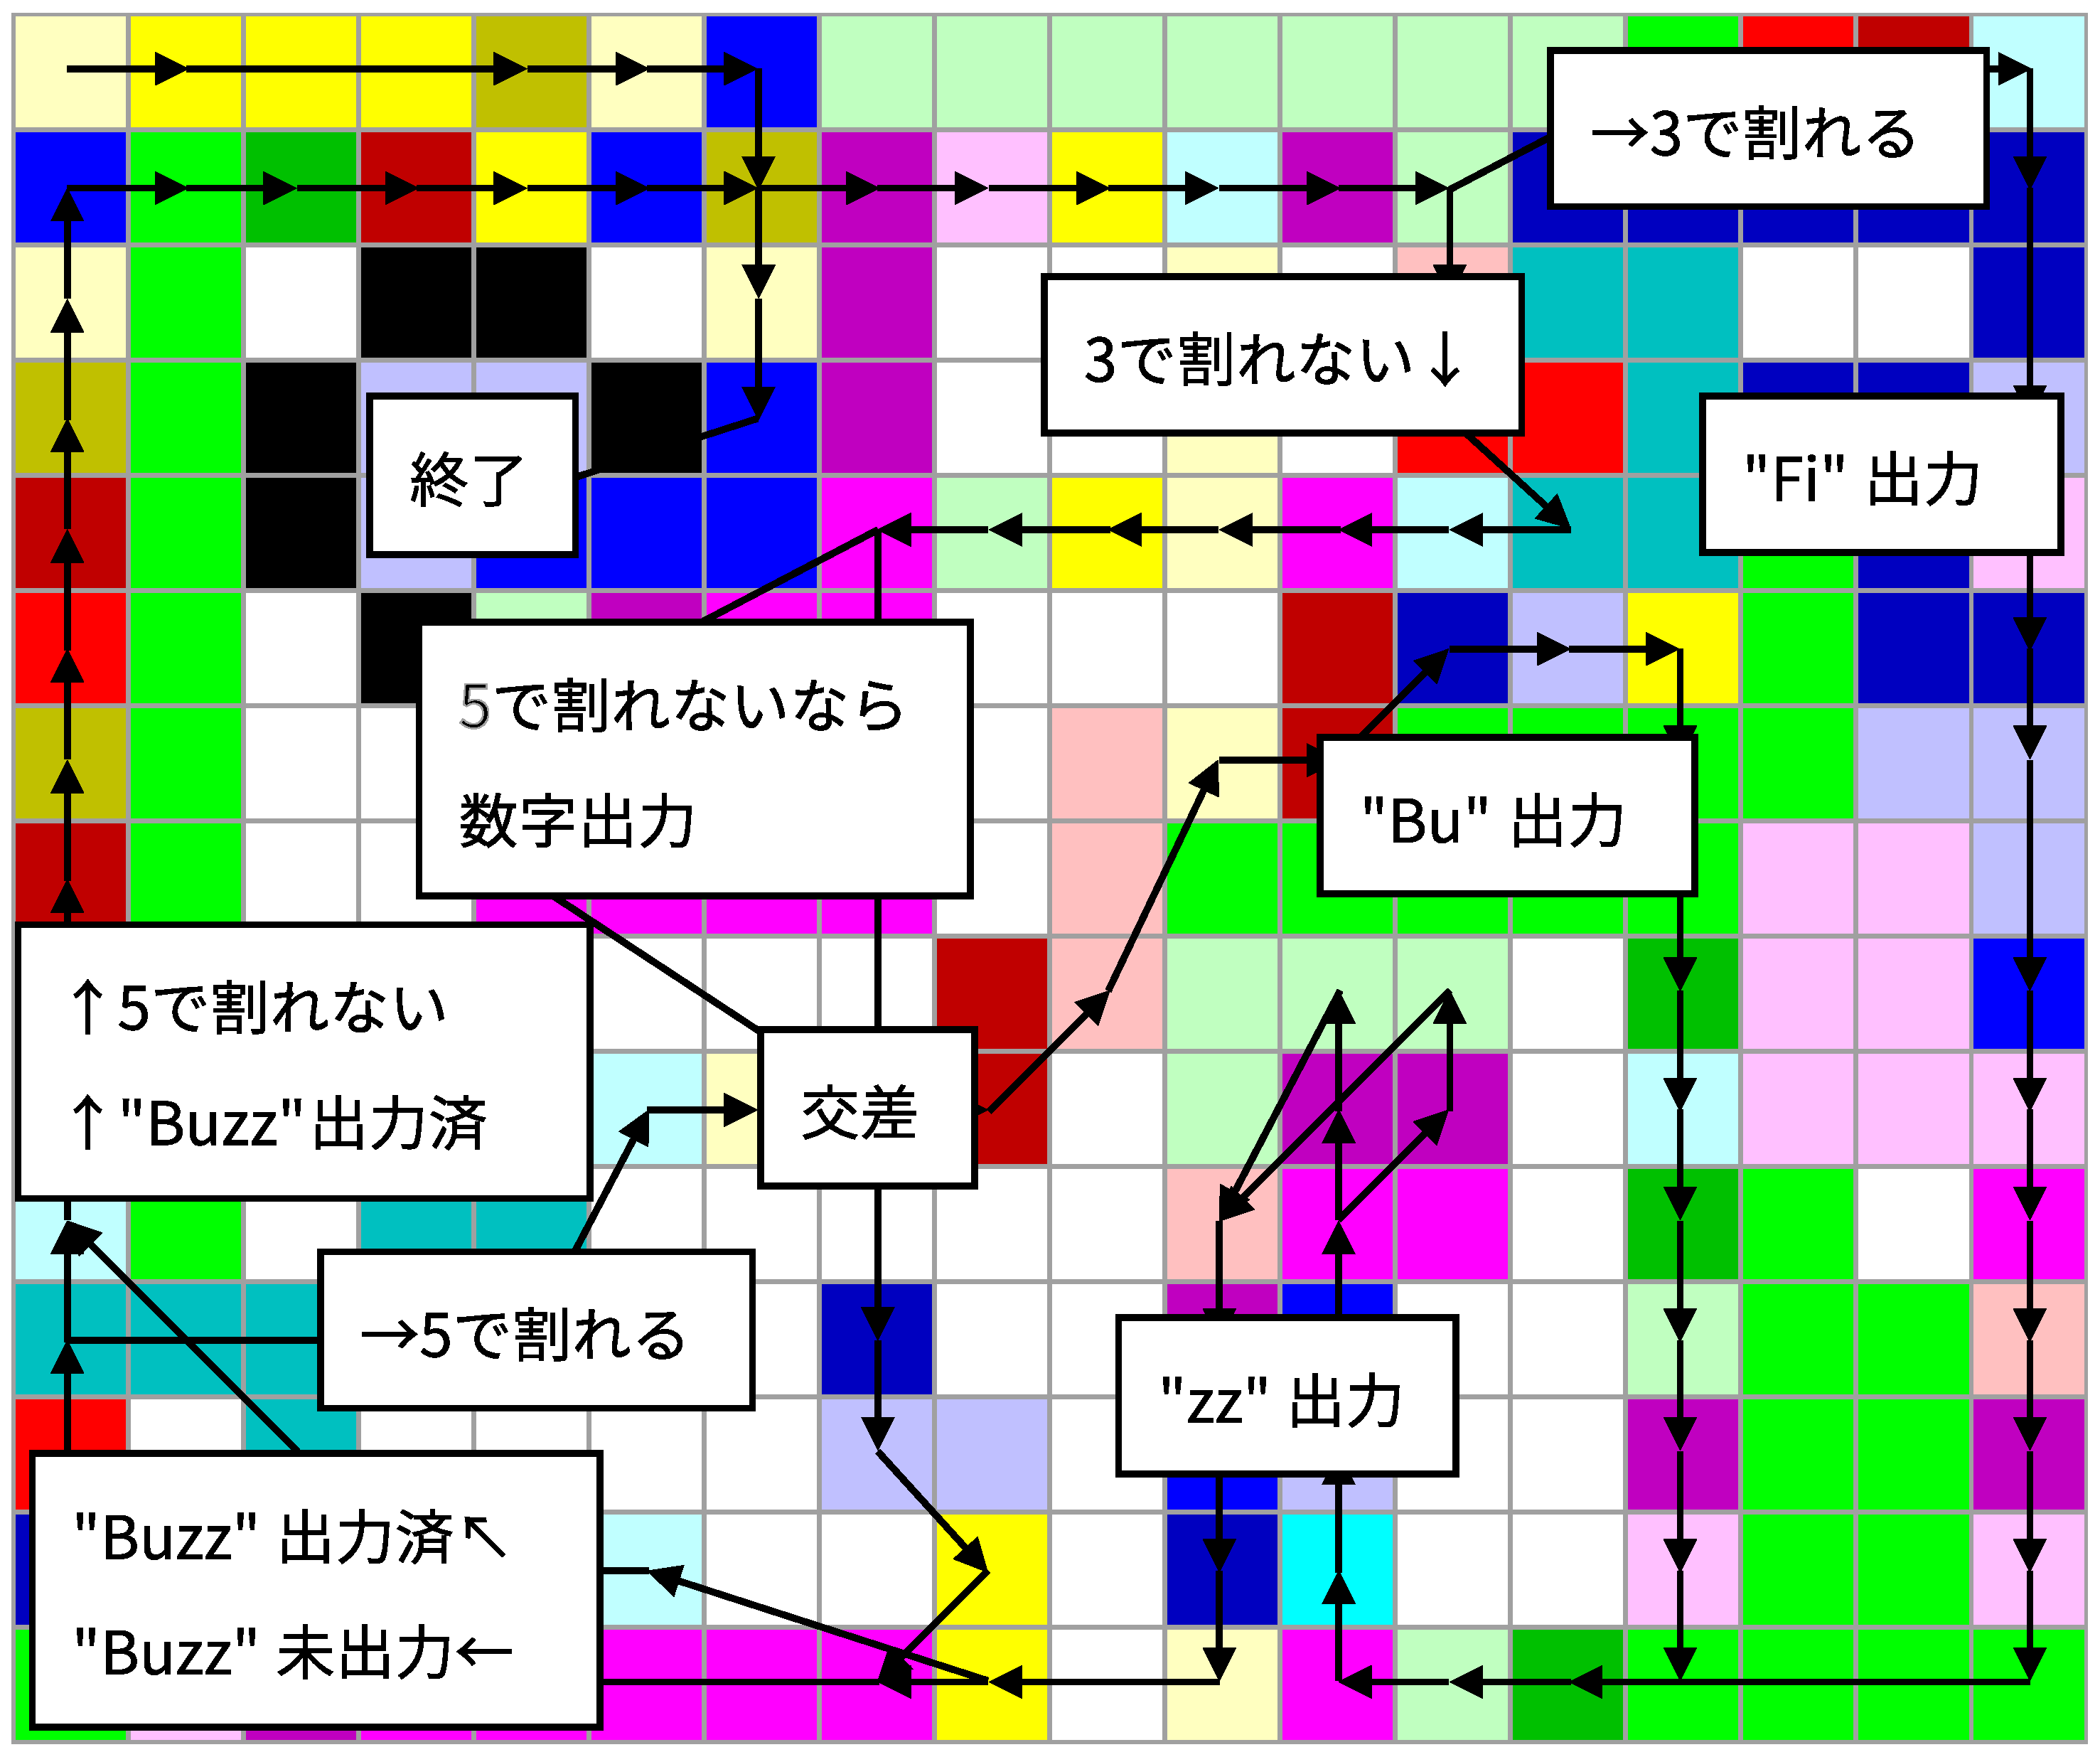
\includegraphics[width=0.6\linewidth]{fizzbuzz_explain.eps}
\end{center}

\begin{itemize}
  \item 上の方で3で割れるか調べる。
  \begin{itemize}
    \item 3で割れたら、右端のルートに行って右下までで "Fi" 、下の方で "zz" を出力。
    \item 3で割れなかったら、真ん中を縦断しながら5で割れるか調べ、割れなかったら数字を出力。
  \end{itemize}
  \item 下の方で一旦合流する。
  \begin{itemize}
    \item "Buzz" を出力済みなら\footnote{"Buzz" が出力済みかどうかの判定をCCが右か左かで行っているのがミソです。}、左端を上がるルートに進む。
    \item "Buzz" 未出力なら、5で割れるか調べる。
    \begin{itemize}
      \item 5で割れたら、ソースコードの真ん中を右上の方に横切りながら "Bu" を出力、右下で "Fi" のルートと合流して下の方で "zz" と出力。
      \item 5で割れなかったら、左端を上がるルートに進む。
    \end{itemize}
  \end{itemize}
  \item 左端を上がりながらカウントアップや100との比較を行う。
  \begin{itemize}
    \item 100を超えていたら終了。
    \item 100以下だったら上の方で合流して始めに戻る。
  \end{itemize}
\end{itemize}

……という流れです。やっぱりややこしい。どうしても面積を取る文字出力をギリギリまで共通化した結果なのですが、まあこれもゴルフの宿命でしょうか。今回はGoToがぐちゃぐちゃに絡み合ってる状態\footnote{スパゲティはネタ言語にとどめましょう}なのですが、Pietはゆとりをもってコードを描くとループがひと目でわかります。

\section{まとめ}
そんなこんなで、結構実用性の高いPiet IDEができたと思います。ただまあいかんせんExcelで、いかんせんVBAなので、デバッグがとろいわ、たまにハングアップするわ、コードは汚いわと散々なので、UXを引き継ぎつつ他の環境に移植できたらななんて思っています。あとExcelのセル範囲をepsに変換するのが思った以上にしんどかったのでもう2度とExcelネタはやりません。